\documentclass[12pt]{article}
\usepackage[utf8]{inputenc}
\usepackage[utf8]{inputenc}
\usepackage{amsmath}
\usepackage{amsthm}
\usepackage{geometry}
\usepackage{amsfonts}
\usepackage{mathrsfs}
\usepackage{bm}
\usepackage{hyperref}
\usepackage[dvipsnames]{xcolor}
\usepackage[inline]{enumitem}
\usepackage{mathtools}
\usepackage{changepage}
\usepackage{graphicx}
\usepackage{caption}
\usepackage{subcaption}
\usepackage{lipsum}
\usepackage{tikz}
\usetikzlibrary{matrix, patterns, decorations.pathreplacing, calligraphy}
\usepackage{tikz-cd}
\usepackage[nameinlink]{cleveref}
\geometry{
headheight=15pt,
left=60pt,
right=60pt
}
\setlength{\emergencystretch}{20pt}
\usepackage{fancyhdr}
\pagestyle{fancy}
\fancyhf{}
\lhead{}
\chead{Section 4.4 Exercises}
\rhead{\thepage}
\hypersetup{
    colorlinks=true,
    linkcolor=blue,
    urlcolor=blue
}

\theoremstyle{definition}
\newtheorem*{remark}{Remark}

\newtheoremstyle{exercise}
    {}
    {}
    {}
    {}
    {\bfseries}
    {.}
    { }
    {\thmname{#1}\thmnumber{#2}\thmnote{ (#3)}}
\theoremstyle{exercise}
\newtheorem{exercise}{Exercise 4.4.}

\newtheoremstyle{solution}
    {}
    {}
    {}
    {}
    {\itshape\color{magenta}}
    {.}
    { }
    {\thmname{#1}\thmnote{ #3}}
\theoremstyle{solution}
\newtheorem*{solution}{Solution}

\Crefformat{exercise}{#2Exercise 4.4.#1#3}

\newcommand{\interior}[1]{%
  {\kern0pt#1}^{\mathrm{o}}%
}
\newcommand{\ts}{\textsuperscript}
\newcommand{\setcomp}[1]{#1^{\mathsf{c}}}
\newcommand{\quand}{\quad \text{and} \quad}
\newcommand{\N}{\mathbf{N}}
\newcommand{\Z}{\mathbf{Z}}
\newcommand{\Q}{\mathbf{Q}}
\newcommand{\I}{\mathbf{I}}
\newcommand{\R}{\mathbf{R}}
\newcommand{\C}{\mathbf{C}}

\DeclarePairedDelimiter\abs{\lvert}{\rvert}
% Swap the definition of \abs* and \norm*, so that \abs
% and \norm resizes the size of the brackets, and the 
% starred version does not.
\makeatletter
\let\oldabs\abs
\def\abs{\@ifstar{\oldabs}{\oldabs*}}
%
\let\oldnorm\norm
\def\norm{\@ifstar{\oldnorm}{\oldnorm*}}
\makeatother

\setlist[enumerate,1]{label={(\alph*)}}

\begin{document}

\section{Section 4.4 Exercises}

Exercises with solutions from Section 4.4 of \hyperlink{ua}{[UA]}.

\begin{exercise}
\label{ex:1}
    \begin{enumerate}
        \item Show that \( f(x) = x^3 \) is continuous on all of \( \R \).

        \item Argue, using Theorem 4.4.5, that \( f \) is not uniformly continuous on \( \R \).

        \item Show that \( f \) is uniformly continuous on any bounded subset of \( \R \).
    \end{enumerate}
\end{exercise}

\begin{solution}
    \begin{enumerate}
        \item As Example 4.3.5 shows, any polynomial is continuous on all of \( \R \).

        \item Define sequences \( (x_n) \) and \( (y_n) \) by \( x_n = n + \tfrac{1}{n} \) and \( y_n = n \). Then
        \[
            \abs{x_n - y_n} = \tfrac{1}{n} \to 0 \quand \abs{f(x_n) - f(y_n)} = 3n + \tfrac{3}{n} + \tfrac{1}{n^3} > 3.
        \]
        Theorem 4.4.5 allows us to conclude that \( f \) is not uniformly continuous on \( \R \).

        \item Suppose that \( A \subseteq \R \) is a bounded subset of \( \R \), so that there is an \( M > 0 \) such that \( A \subseteq [-M, M] \). For any \( x, y \in A \), it follows that
        \[
            \abs{x^2 + xy + y^2} \leq \abs{x}^2 + \abs{x} \abs{y} + \abs{y}^2 \leq 3M^2.
        \]
        Let \( \epsilon > 0 \) be given and set \( \delta = \tfrac{\epsilon}{3M^2} \). For any \( x, y \in A \) we then have
        \[
            \abs{x^3 - y^3} = \abs{x - y} \abs{x^2 + xy + y^2} \leq 3M^2 \delta = \epsilon.
        \]
        Thus \( f \) is uniformly continuous on \( A \).
    \end{enumerate}
\end{solution}

\begin{exercise}
\label{ex:2}
    \begin{enumerate}
        \item Is \( f(x) = 1 / x \) uniformly continuous on \( (0, 1) \)?

        \item Is \( g(x) = \sqrt{x^2 + 1} \) uniformly continuous on \( (0, 1) \)?

        \item Is \( h(x) = x \sin (1 / x) \) uniformly continuous on \( (0, 1) \)?
    \end{enumerate}
\end{exercise}

\begin{solution}
    \begin{enumerate}
        \item Define sequences \( (x_n) \) and \( (y_n) \) by \( x_n = \tfrac{1}{n} \) and \( y_n = \tfrac{1}{n+1} \). Then
        \[
            \abs{x_n - y_n} = \tfrac{1}{n} - \tfrac{1}{n+1} \to 0 \quand \abs{f(x_n) - f(y_n)} = 1.
        \]
        Theorem 4.4.5 allows us to conclude that \( f \) is not uniformly continuous on \( \R \).

        \item If a function is uniformly continuous on some \( B \subseteq \R \), then it is also uniformly continuous on any subset \( A \subseteq B \). The function \( g(x) = \sqrt{x^2 + 1} \) is continuous on all of \( \R \), hence uniformly continuous on the compact set \( [0, 1] \) (Theorem 4.4.7), and hence uniformly continuous on the subset \( (0, 1) \).

        \item Define \( h : \R \to \R \) by
        \[
            h(x) = \begin{cases}
                x \sin (1/x) & \text{if } x \neq 0, \\
                0 & \text{if } x = 0.
            \end{cases}
        \]
        The continuity of \( h \) away from the origin is clear. As shown in Example 4.3.6, \( h \) is also continuous at the origin and thus continuous on all of \( \R \). It follows that \( h \) is uniformly continuous on the compact set \( [0, 1] \) (Theorem 4.4.7) and hence uniformly continuous on the subset \( (0,1) \).
    \end{enumerate}
\end{solution}

\begin{exercise}
\label{ex:3}
    Show that \( f(x) = 1/x^2 \) is uniformly continuous on the set \( [1, \infty) \) but not on the set \( (0, 1] \).
\end{exercise}

\begin{solution}
    For any \( x, y \in [1, \infty) \), we have
    \[
        \abs{\frac{1}{x^2} - \frac{1}{y^2}} = \abs{\frac{y^2 - x^2}{x^2 y^2}} = \frac{x + y}{x^2 y^2} \abs{x - y} = \left( \frac{1}{x y^2} + \frac{1}{x^2 y} \right) \abs{x - y} \leq 2 \abs{x - y}.
    \]
    Let \( \epsilon > 0 \) be given and set \( \delta = \tfrac{\epsilon}{2} \). For any \( x, y \in [1, \infty) \) such that \( \abs{x - y} < \delta \), we then have
    \[
        \abs{\frac{1}{x^2} - \frac{1}{y^2}} \leq 2 \abs{x - y} < 2 \delta = \epsilon.
    \]
    Thus \( f \) is uniformly continuous on \( [1, \infty) \).

    Define the sequences \( (x_n) \) and \( (y_n) \) in \( (0, 1] \) by \( x_n = \tfrac{1}{\sqrt{n}} \) and \( y_n = \tfrac{1}{\sqrt{n+1}} \). Then
    \[
        \abs{x_n - y_n} = \tfrac{1}{\sqrt{n}} - \tfrac{1}{\sqrt{n+1}} \to 0 \quand \abs{f(x_n) - f(y_n)} = 1.
    \]
    It follows from Theorem 4.4.5 that \( f \) is not uniformly continuous on \( (0, 1] \).
\end{solution}

\begin{exercise}
\label{ex:4}
    Decide whether each of the following statements is true or false, justifying each conclusion.
    \begin{enumerate}
        \item If \( f \) is continuous on \( [a, b] \) with \( f(x) > 0 \) for all \( a \leq x \leq b \), then \( 1/f \) is bounded on \( [a, b] \) (meaning \( 1/f\) has bounded range).

        \item If \( f \) is uniformly continuous on a bounded set \( A \), then \( f(A) \) is bounded.

        \item If \( f \) is defined on \( \R \) and \( f(K) \) is compact whenever \( K \) is compact, then \( f \) is continuous on \( \R \).
    \end{enumerate}
\end{exercise}

\begin{solution}
    \begin{enumerate}
        \item This is true. Since \( f \) is continuous on the compact set \( [a, b] \), Theorem 4.4.2 implies that there exist \( x_0, x_1 \in [a, b] \) such that \( f(x_0) \leq f(x) \leq f(x_1) \) for all \( x \in [a, b] \). By assumption we have \( f(x_0) > 0 \) and so
        \[
            0 < f(x_0) \leq f(x) \leq f(x_1) \iff 0 < \frac{1}{f(x_1)} \leq \frac{1}{f(x)} \leq \frac{1}{f(x_0)}
        \]
        for all \( x \in [a, b] \), i.e.\ \( 1/f \) is bounded on \( [a, b] \).

        \item This is true. Since \( A \) is bounded, there is a \( K > 0 \) such that \( A \subseteq [-K, K] \), and since \( f \) is uniformly continuous on \( A \), there is a \( \delta > 0 \) such that
        \[
            x, y \in A \text{ and } \abs{x - y} < \delta \implies \abs{f(x) - f(y)} < 1.
        \]
        Let \( N \in \N \) be such that \( \tfrac{2K}{N} < \delta \) and for each \( j \in \{ 1, 2, \ldots, N \} \) define
        \[
            I_j = \left[ -K + (j - 1) \frac{2K}{N}, -K + j \frac{2K}{N} \right],
        \]
        so that \( I_1 \cup \cdots \cup I_N = [-K, K] \). For \( j \in \{ 1, 2, \ldots, N \} \), if \( I_j \cap A \neq \emptyset \), then there exists some \( a_j \in I_j \cap A \). Let
        \[
            M = \max \left\{ 1 + \abs{f(a_j)} : j \in \{ 1, 2, \ldots, N \} \text{ and } I_j \cap A \neq \emptyset \right\};
        \]
        we are justified in taking the maximum of this set as it is finite and must be non-empty, since if \( A \) is non-empty (which we may as well assume) there must be some \( j \) such that \( I_j \cap A \neq \emptyset \).

        Suppose \( x \in A \). Then since \( I_1 \cup \cdots \cup I_N = [-K, K] \) and \( A \subseteq [-K, K] \), there must be some \( j \in \{ 1, 2, \ldots, N \} \) such that \( x \in I_j \cap A \). Since \( x, a_j \in I_j \cap A \), we then have \( \abs{x - a_j} \leq \abs{I_j} = \tfrac{2K}{N} < \delta \) and thus
        \[
            \abs{f(x) - f(a_j)} < 1 \implies \abs{f(x)} < 1 + \abs{f(a_j)} \leq M.
        \]
        It follows that \( f(A) \subseteq [-M, M] \), i.e.\ that \( f(A) \) is bounded.

        \item This is false. Let \( f : \R \to \R \) be Dirichlet's function, i.e.\
        \[
            f(x) = \begin{cases}
                1 & \text{if } x \in \Q, \\
                0 & \text{if } x \not\in \Q.
            \end{cases}
        \]
        Then for any subset \( A \subseteq \R \), the only possibilities for \( f(A) \) are \( \emptyset, \{ 0 \}, \{ 1 \}, \) and \( \{ 0, 1 \} \); each of these is compact. However, \( f \) is nowhere-continuous.
    \end{enumerate}
\end{solution}

\begin{exercise}
\label{ex:5}
    Assume that \( g \) is defined on an open interval \( (a, c) \) and it is known to be uniformly continuous on \( (a, b] \) and \( [b, c) \), where \( a < b < c \). Prove that \( g \) is uniformly continuous on \( (a, c) \).
\end{exercise}

\begin{solution}
    Let \( \epsilon > 0 \) be given. There exist \( \delta_1, \delta_2 > 0 \) such that
    \begin{gather*}
        x, y \in (a, b] \text{ and } \abs{x - y} < \delta_1 \implies \abs{g(x) - g(y)} < \tfrac{\epsilon}{2}, \\
        x, y \in [b, c) \text{ and } \abs{x - y} < \delta_2 \implies \abs{g(x) - g(y)} < \tfrac{\epsilon}{2}.
    \end{gather*}
    Set \( \delta = \min \{ \delta_1, \delta_2 \} \) and suppose that \( x, y \in (a, c) \) are such that \( \abs{x - y} < \delta \). There are four cases.
    \begin{description}
        \item[Case 1.] If \( x, y \in (a, b] \), then since \( \abs{x - y} < \delta \leq \delta_1 \), we have \( \abs{g(x) - g(y)} < \tfrac{\epsilon}{2} < \epsilon \).
        
        \item[Case 2.] If \( x, y \in [b, c) \), then since \( \abs{x - y} < \delta \leq \delta_2 \), we have \( \abs{g(x) - g(y)} < \tfrac{\epsilon}{2} < \epsilon \).

        \item[Case 3.] If \( x \in (a, b] \) and \( y \in [b, c) \), then note that \( \abs{x - b} \leq \abs{x - y} < \delta \leq \delta_1 \) and \( \abs{b - y} \leq \abs{x - y} < \delta \leq \delta_2 \). It follows that \( \abs{g(x) - g(b)} < \tfrac{\epsilon}{2} \) and that \( \abs{g(b) - g(y)} < \tfrac{\epsilon}{2} \), which gives us
        \[
            \abs{g(x) - g(y)} \leq \abs{g(x) - g(b)} + \abs{g(b) - g(y)} < \tfrac{\epsilon}{2} + \tfrac{\epsilon}{2} = \epsilon.
        \]

        \item[Case 4.] The case where \( x \in [b, c) \) and \( y \in (a, b] \) is handled similarly to Case 3.
    \end{description}
    In any case, we have \( \abs{g(x) - g(y)} < \epsilon \). It follows that \( g \) is uniformly continuous on \( (a, c) \).
\end{solution}

\begin{exercise}
\label{ex:6}
    Give an example of each of the following, or state that such a request is impossible. For any that are impossible, supply a short explanation for why this is the case.
    \begin{enumerate}
        \item A continuous function \( f : (0, 1) \to \R \) and a Cauchy sequence \( (x_n) \) such that \( f(x_n) \) is not a Cauchy sequence;

        \item A uniformly continuous function \( f : (0, 1) \to \R \) and a Cauchy sequence \( (x_n) \) such that \( f(x_n) \) is not a Cauchy sequence;

        \item A continuous function \( f : [0, \infty) \to \R \) and a Cauchy sequence \( (x_n) \) such that \( f(x_n) \) is not a Cauchy sequence.
    \end{enumerate}
\end{exercise}

\begin{solution}
    \begin{enumerate}
        \item Let \( f : (0, 1) \to \R \) be given by \( f(x) = \tfrac{1}{x} \) and consider the Cauchy sequence \( (x_n) \subseteq (0, 1) \) given by \( x_n = \tfrac{1}{n+1} \). Then \( f(x_n) = n + 1 \) which is not convergent and hence not Cauchy.

        \item This is impossible, as we will show in \Cref{ex:13} (a).

        \item This is impossible. Let \( f : [0, \infty) \to \R \) be continuous on its domain and let \( (x_n) \subseteq [0, \infty) \) be a Cauchy sequence; equivalently, \( (x_n) \) is a convergent sequence, say \( \lim x_n = x \). Since \( [0, \infty) \) is a closed set, we must have \( x \in [0, \infty) \), and then since \( f \) is continuous on its domain, it must be continuous at \( x \). It follows that \( \lim f(x_n) = f(x) \) and hence that \( (f(x_n)) \) is a Cauchy sequence.
    \end{enumerate}
\end{solution}

\begin{exercise}
\label{ex:7}
    Prove that \( f(x) = \sqrt{x} \) is uniformly continuous on \( [0, \infty) \).
\end{exercise}

\begin{solution}
    \( f \) is continuous on the compact set \( [0, 1] \) and hence is uniformly continuous on \( [0, 1] \) (Theorem 4.4.7). Note that for any \( x, y \in [1, \infty) \) we have
    \[
        \abs{\sqrt{x} - \sqrt{y}} = \frac{\abs{x - y}}{\sqrt{x} + \sqrt{y}} \leq \tfrac{1}{2} \abs{x - y}.
    \]
    It is now straightforward to show that \( f \) is uniformly continuous on \( [1, \infty) \) (see \Cref{ex:9}). By an argument analogous to the one given in \Cref{ex:5}, we may now conclude that \( f \) is uniformly continuous on \( [0, \infty) \).
\end{solution}

\begin{exercise}
\label{ex:8}
    Give an example of each of the following, or provide a short argument for why the request is impossible.
    \begin{enumerate}
        \item A continuous function defined on \( [0, 1] \) with range \( (0, 1) \).

        \item A continuous function defined on \( (0, 1) \) with range \( [0, 1] \).

        \item A continuous function defined on \( (0, 1] \) with range \( (0, 1) \).
    \end{enumerate}
\end{exercise}

\begin{solution}
    \begin{enumerate}
        \item This is impossible. If \( f : [0, 1] \to \R \) is continuous, then since \( [0, 1] \) is compact, the image of \( f \) must be compact (Theorem 4.4.1). However, \( (0, 1) \) is not a compact set.

        \item Consider \( f : (0, 1) \to \R \) given by \( f(x) = \tfrac{1}{2} \sin (2 \pi x) + \tfrac{1}{2} \); the image of \( f \) is then \( [0, 1] \) (see \Cref{fig:1}).

        \item Consider \( f : (0, 1] \to \R \) given by \( f(x) = \tfrac{1}{2} (1 - x) \sin \left( \tfrac{1}{x} \right) + \tfrac{1}{2} \); the image of \( f \) is then \( (0, 1) \) (see \Cref{fig:1}).
    \end{enumerate}
\end{solution}

\begin{figure}[t]
    \centering
    \begin{subfigure}{.5\textwidth}
      \centering
      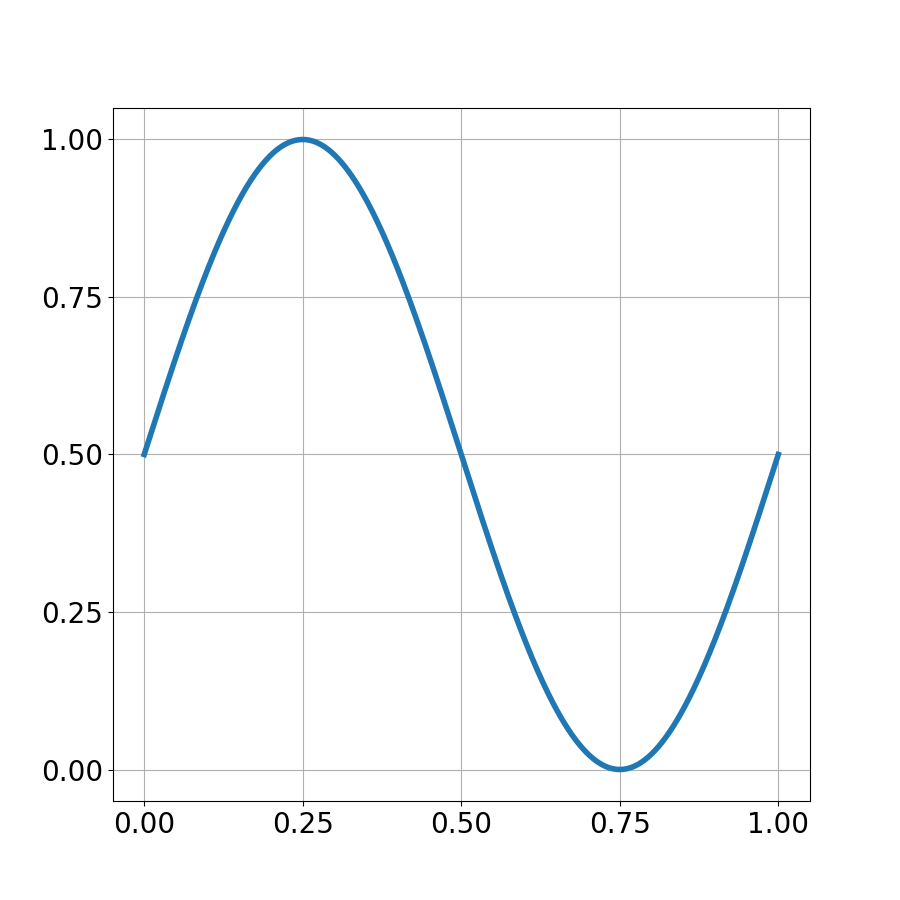
\includegraphics[width=\linewidth]{UA_Section_4_4_Figure_1.png}
      \caption{\( \tfrac{1}{2} \sin (2 \pi x) + \tfrac{1}{2} \) on \( (0, 1) \)}
      \label{fig:1sub1}
    \end{subfigure}%
    \begin{subfigure}{.5\textwidth}
      \centering

      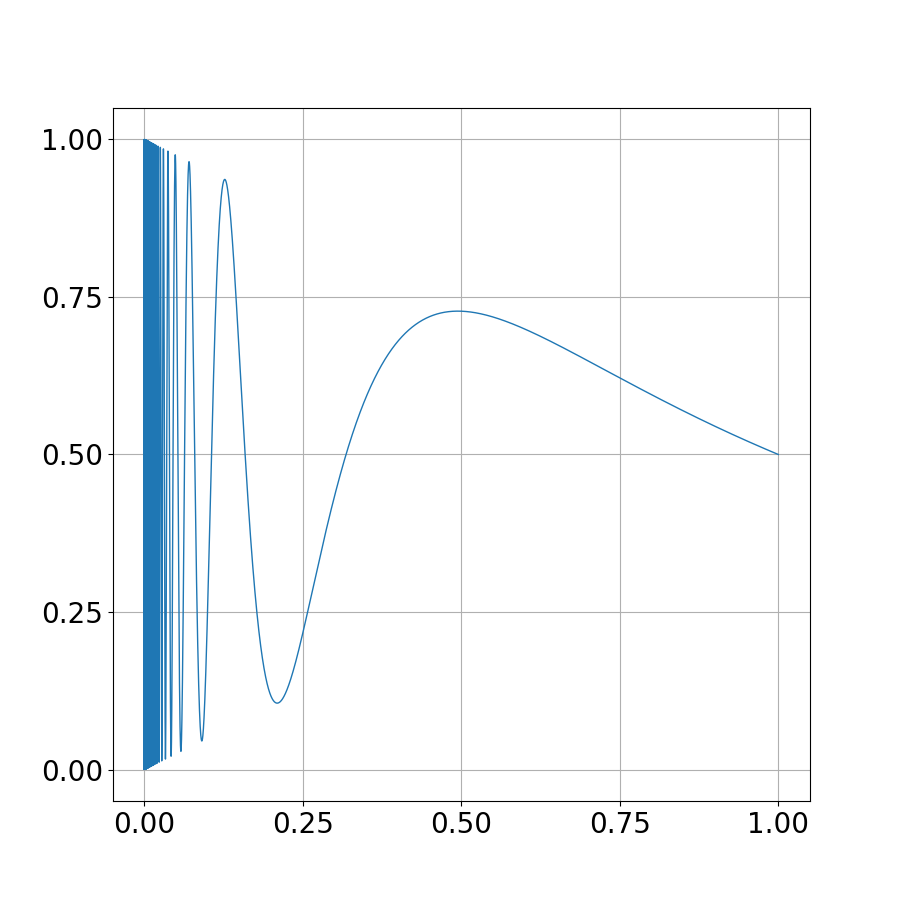
\includegraphics[width=\linewidth]{UA_Section_4_4_Figure_2.png}
      \caption{\( \tfrac{1}{2} (1 - x) \sin \left( \tfrac{1}{x} \right) + \tfrac{1}{2} \) on \( (0, 1] \)}
      \label{fig:1sub2}
    \end{subfigure}
    \caption{\Cref{ex:8} function graphs}
    \label{fig:1}
\end{figure}

\newpage

\begin{exercise}[Lipschitz Functions]
\label{ex:9}
    A function \( f : A \to \R \) is called \textit{Lipschitz} if there exists a bound \( M > 0 \) such that
    \[
        \abs{\frac{f(x) - f(y)}{x - y}} \leq M
    \]
    for all \( x \neq y \in A \). Geometrically speaking, a function \( f \) is Lipschitz if there is a uniform bound on the magnitude of the slopes of lines drawn through any two points on the graph of \( f \).
    \begin{enumerate}
        \item Show that if \( f : A \to \R \) is Lipschitz, then it is uniformly continuous on \( A \).

        \item Is the converse statement true? Are all uniformly continuous functions necessarily Lipschitz?
    \end{enumerate}
\end{exercise}

\begin{solution}
    \begin{enumerate}
        \item Since \( f \) is Lipschitz, there is an \( M > 0 \) such that
        \[
            \abs{f(x) - f(y)} \leq M \abs{x - y}
        \]
        for all \( x, y \in A \). Let \( \epsilon > 0 \) be given and set \( \delta = \tfrac{\epsilon}{M} \). Then for any \( x, y \in A \) satisfying \( \abs{x - y} < \delta \), we have
        \[
            \abs{f(x) - f(y)} \leq M \abs{x - y} < M \delta = \epsilon.
        \]
        It follows that \( f \) is uniformly continuous on \( A \).

        \item The converse statement is not true. Consider \( f : [0, \infty) \to \R \) given by \( f(x) = \sqrt{x} \). As we showed in \Cref{ex:7}, this function is uniformly continuous on \( [0, \infty) \). However, we claim that \( f \) is not Lipschitz on \( [0, \infty) \). To show this, for each \( M > 0 \) we need to find some \( x \neq y \in [0, \infty) \) such that
        \[
            \abs{\frac{f(x) - f(y)}{x - y}} > M.
        \]
        So, for \( M > 0 \), let \( x = \tfrac{1}{4M^2} \) and \( y = 0 \). Then
        \[
            \abs{\frac{f(x) - f(y)}{x - y}} = \abs{\frac{\tfrac{1}{2M}}{\tfrac{1}{4M^2}}} = 2M > M.
        \]
    \end{enumerate}
\end{solution}

\begin{exercise}
\label{ex:10}
    Assume that \( f \) and \( g \) are uniformly continuous functions defined on a common domain \( A \). Which of the following combinations are necessarily uniformly continuous on \( A \):
    \[
        f(x) + g(x), \quad f(x)g(x), \quad \frac{f(x)}{g(x)}, \quad f(g(x)) \, ?
    \]
    (Assume that the quotient and the composition are properly defined and thus at least continuous.)
\end{exercise}

\begin{solution}
    We claim that \( f + g \) is uniformly continuous on \( A \). To see this, let \( \epsilon > 0 \) be given. There exist \( \delta_1, \delta_2 > 0 \) such that
    \begin{gather*}
        x, y \in A \text{ and } \abs{x - y} < \delta_1 \implies \abs{f(x) - f(y)} < \tfrac{\epsilon}{2}, \\[2mm]
        x, y \in A \text{ and } \abs{x - y} < \delta_2 \implies \abs{g(x) - g(y)} < \tfrac{\epsilon}{2}.
    \end{gather*}
    Let \( \delta = \min \{ \delta_1, \delta_2 \} \) and observe that for any \( x, y \in A \) satisfying \( \abs{x - y} < \delta \), we then have
    \[
        \abs{f(x) + g(x) - f(y) - g(y)} \leq \abs{f(x) - f(y)} + \abs{g(x) - g(y)} < \tfrac{\epsilon}{2} + \tfrac{\epsilon}{2} = \epsilon.
    \]
    Thus \( f + g \) is uniformly continuous on \( A \).

    The product \( fg \) need not be uniformly continuous. For a counterexample, consider \( f, g : \R \to \R \) given by \( f(x) = g(x) = x \). This function is clearly Lipschitz and hence uniformly continuous on all of \( \R \) (\Cref{ex:9}). However, the product \( f(x)g(x) = x^2 \) is not uniformly continuous on \( \R \); this can be seen using the same sequences as in \Cref{ex:1} (b) and appealing to Theorem 4.4.5.

    The quotient \( \tfrac{f}{g} \) need not be uniformly continuous. For a counterexample, consider \( f, g : (0, 1] \to \R \) given by \( f(x) = 1 \) and \( g(x) = x \). Both are uniformly continuous, but the quotient \( \tfrac{f(x)}{g(x)} = \tfrac{1}{x} \) is not (\Cref{ex:2} (a)).

    Suppose that \( g(A) \subseteq A \), so that the composition \( f \circ g : A \to \R \) is well-defined. We claim that this composition is also uniformly continuous. To see this, let \( \epsilon > 0 \) be given. There exists a \( \delta_2 > 0 \) such that
    \[
        s, t \in A \text{ and } \abs{s - t} < \delta_2 \implies \abs{f(s) - f(t)} < \epsilon.
    \]
    There then exists a \( \delta_1 > 0 \) such that
    \[
        x, y \in A \text{ and } \abs{x - y} < \delta_1 \implies \abs{g(x) - g(y)} < \delta_2.
    \]
    By assumption, if \( x, y \in A \) then \( g(x), g(y) \in A \). Thus
    \begin{multline*}
        x, y \in A \text{ and } \abs{x - y} < \delta_1 \implies g(x), g(y) \in A \text{ and } \abs{g(x) - g(y)} < \delta_2 \\
        \implies \abs{f(g(x)) - f(g(y))} < \epsilon.
    \end{multline*}
    Thus \( f \circ g \) is uniformly continuous on \( A \).
\end{solution}

\begin{exercise}[Topological Characterization of Continuity]
\label{ex:11}
    Let \( g \) be defined on all of \( \R \). If \( B \) is a subset of \( \R \), define the set \( g^{-1}(B) \) by
    \[
        g^{-1}(B) = \{ x \in \R : g(x) \in B \}.
    \]
    Show that \( g \) is continuous if and only if \( g^{-1}(O) \) is open whenever \( O \subseteq \R \) is an open set.
\end{exercise}

\begin{solution}
    Suppose \( g \) is continuous and \( O \subseteq \R \) is an open set. Fix \( c \in g^{-1}(O) \), so that \( g(c) \in O \). Since \( O \) is open, there exists an \( \epsilon > 0 \) such that \( V_{\epsilon}(g(c)) \subseteq O \), and since \( g \) is continuous at \( c \), there is a \( \delta > 0 \) such that \( x \in V_{\delta}(c) \) implies that \( g(x) \in V_{\epsilon}(g(c)) \subseteq O \) (Theorem 4.3.2 (ii)). In other words, any \( x \in V_{\delta}(c) \) also belongs to \( g^{-1}(O) \), so that \( V_{\delta}(c) \subseteq g^{-1}(O) \). It follows that \( g^{-1}(O) \) is an open set.

    Now suppose that \( g^{-1}(O) \) is open whenever \( O \subseteq \R \) is an open set. Fix \( c \in \R \) and let \( \epsilon > 0 \) be given. The set \( V_{\epsilon}(g(c)) \) is open, so by assumption the set \( g^{-1}[V_{\epsilon}(g(c))] \) is also open. Certainly we have \( c \in g^{-1}[V_{\epsilon}(g(c))] \), so there exists a \( \delta > 0 \) such that \( V_{\delta}(c) \subseteq g^{-1}[V_{\epsilon}(g(c))] \). It follows that if \( x \in V_{\delta}(c) \), then \( g(x) \in V_{\epsilon}(g(c)) \) and so Theorem 4.3.2 (ii) allows us to conclude that \( g \) is continuous at each \( c \in \R \).
\end{solution}

\begin{exercise}
\label{ex:12}
    Review \Cref{ex:11}, and then determine which of the following statements is true about a continuous function defined on \( \R \):
    \begin{enumerate}
        \item \( f^{-1}(B) \) is finite whenever \( B \) is finite.

        \item \( f^{-1}(K) \) is compact whenever \( K \) is compact.

        \item \( f^{-1}(A) \) is bounded whenever \( A \) is bounded.

        \item \( f^{-1}(F) \) is closed whenever \( F \) is closed.
    \end{enumerate}
\end{exercise}

\begin{solution}
    \begin{enumerate}
        \item This is false. Consider the function \( f : \R \to \R \) given by \( f(x) = 0 \). Then \( f^{-1}(\{ 0 \}) = \R \).

        \item This is false; see part (a) for a counterexample.

        \item This is false; see part (a) for a counterexample.

        \item This is true. If \( F \) is closed, then \( \setcomp{F} \) is open. Since \( f \) is continuous, we have that \( f^{-1}(\setcomp{F}) \) is also open (\Cref{ex:11}). It follows that \( \setcomp{(f^{-1}(\setcomp{F}))} \) is closed. This set is nothing but \( f^{-1}(F) \):
        \[
            x \in \setcomp{(f^{-1}(\setcomp{F}))} \iff x \not\in f^{-1}(\setcomp{F}) \iff f(x) \not\in \setcomp{F} \iff f(x) \in F \iff x \in f^{-1}(F).
        \]
    \end{enumerate}
\end{solution}

\begin{exercise}[Continuous Extension Theorem]
\label{ex:13}
    \begin{enumerate}
        \item Show that a uniformly continuous function preserves Cauchy sequences; that is, if \( f : A \to \R \) is uniformly continuous and \( (x_n) \subseteq A \) is a Cauchy sequence, then show \( f(x_n) \) is a Cauchy sequence.

        \item Let \( g \) be a continuous function on the open interval \( (a, b) \). Prove that \( g \) is uniformly continuous on \( (a, b) \) if and only if it is possible to define values \( g(a) \) and \( g(b) \) at the endpoints so that the extended function \( g \) is continuous on \( [a, b] \). (In the forward direction, first produce candidates for \( g(a) \) and \( g(b) \), and then show the extended \( g \) is continuous.)
    \end{enumerate}
\end{exercise}

\begin{solution}
    \begin{enumerate}
        \item Let \( \epsilon > 0 \) be given. Since \( f \) is uniformly continuous, there is a \( \delta > 0 \) such that for any \( x, y \in A \) satisfying \( \abs{x - y} < \delta \), we have \( \abs{f(x) - f(y)} < \epsilon \). Since \( (x_n) \subseteq A \) is a Cauchy sequence, there is an \( N \in \N \) such that for all \( n > m \geq N \), we have \( \abs{x_n - x_m} < \delta \), which implies that \( \abs{f(x_n) - f(x_m)} < \epsilon \). Thus \( (f(x_n)) \) is also a Cauchy sequence.

        \item Suppose that \( g \) is uniformly continuous on \( (a, b) \). Define a sequence \( a_n = a + \tfrac{b - a}{2n} \), so that \( (a_n) \subseteq (a, b) \) and \( \lim a_n = a \). Then since \( (a_n) \) is Cauchy, part (a) implies that the sequence \( (g(a_n)) \) is also Cauchy and hence convergent, say \( \lim g(a_n) = y \in \R \). Define \( g(a) := y \). 
        
        We claim that this extended \( g \) is continuous at \( a \). Let \( (x_n) \subseteq (a, b) \) be a sequence such that \( \lim x_n = a \) and let \( \epsilon > 0 \) be given. Since \( g \) is uniformly continuous on \( (a, b) \), there is a \( \delta > 0 \) such that for any \( x, y \in (a, b) \) satisfying \( \abs{x - y} < \delta \), we have \( \abs{g(x) - g(y)} < \epsilon \). Note that \( \lim \abs{x_n - a_n} = 0 \) since \( \lim x_n = \lim a_n = a \), so there is an \( N \in \N \) such that \( n \geq N \) implies that \( \abs{x_n - a_n} < \delta \), which gives us \( \abs{g(x_n) - g(a_n)} < \epsilon \). Thus \( \lim \abs{g(x_n) - g(a_n)} = 0 \). Combining this with \( \lim g(a_n) = g(a) \), we see that \( \lim g(x_n) = g(a) \) also and hence \( g \) is continuous at \( a \).

        An analogous argument shows that we can also continuously extend \( g \) to be defined at \( b \) by considering the sequence \( b_n = b - \tfrac{b - a}{2n} \).

        For the converse implication, we apply Theorem 4.4.7 to see that \( g \) is uniformly continuous on the compact set \( [a, b] \) and hence uniformly continuous on the subset \( (a, b) \).
    \end{enumerate}
\end{solution}

\begin{exercise}
\label{ex:14}
    Construct an alternate proof of Theorem 4.4.7 using the open cover characterization of compactness from the Heine-Borel Theorem (Theorem 3.3.8 (iii)).
\end{exercise}

\begin{solution}
    Suppose \( f : K \to \R \) is continuous, where \( K \) is compact. Let \( \epsilon > 0 \) be given. Since \( f \) is continuous on \( K \), for each \( t \in K \) there exists a \( \delta_t > 0 \) such that
    \[
        x \in K \text{ and } \abs{x - t} < \delta_t \implies \abs{f(x) - f(t)} < \tfrac{\epsilon}{2}.
    \]
    Observe that the collection \( \{ V_{\delta_t/2}(t) : t \in K \} \) forms an open cover of \( K \). Since \( K \) is compact, there exists a finite subcover \( \{ V_{\delta_{t_1}/2}(t_1), \ldots, V_{\delta_{t_n}/2}(t_n) \} \). Let \( \delta = \min \{ \delta_{t_1}/2, \ldots, \delta_{t_n}/2 \} \) and suppose that \( x, y \in K \) are such that \( \abs{x - y} < \delta \). There is a \( j \in \{ 1, \ldots, n \} \) such that \( x \in V_{\delta_{t_j}/2}(t_j) \), so that \( \abs{x - t_j} < \delta_{t_j}/2 < \delta_{t_j} \) and thus \( \abs{f(x) - f(t_j)} < \tfrac{\epsilon}{2} \). Note that
    \[
        \abs{y - t_j} \leq \abs{x - y} + \abs{x - t_j} < \delta + \delta_{t_j}/2 \leq \delta_{t_j}/2 + \delta_{t_j}/2 = \delta_{t_j}.
    \]
    It follows that \( \abs{f(y) - f(t_j)} < \tfrac{\epsilon}{2} \) and hence that
    \[
        \abs{f(x) - f(y)} \leq \abs{f(x) - f(t_j)} + \abs{f(y) - f(t_j)} < \tfrac{\epsilon}{2} + \tfrac{\epsilon}{2} = \epsilon.
    \]
    Thus \( f \) is uniformly continuous on \( K \).
\end{solution}

\noindent \hrulefill

\noindent \hypertarget{ua}{\textcolor{blue}{[UA]} Abbott, S. (2015) \textit{Understanding Analysis.} 2\ts{nd} edition.}

\end{document}